\documentclass[12pt]{article}
\usepackage[paper=letterpaper,margin=1.5cm]{geometry}
\usepackage{amsmath}
\usepackage{amssymb}
\usepackage{amsfonts}
\usepackage{mathtools}
%\usepackage[utf8]{inputenc}
%\usepackage{newtxtext, newtxmath}
\usepackage{lmodern}     % set math font to Latin modern math
\usepackage[T1]{fontenc}
\renewcommand\rmdefault{ptm}
%\usepackage{enumitem}
\usepackage[shortlabels]{enumitem}
\usepackage{titling}
\usepackage{graphicx}
\usepackage[colorlinks=true]{hyperref}
\usepackage{setspace}
\usepackage{subfigure} 
\usepackage{braket}
\usepackage{color}
\usepackage{tabularx}
\usepackage[table]{xcolor}
\usepackage{listings}
\usepackage{mathrsfs}
\usepackage{stackengine}
\usepackage{physics}
\usepackage{afterpage}
\usepackage{pdfpages}
\usepackage[export]{adjustbox}
\usepackage{biblatex}

\setstackEOL{\\}

\definecolor{dkgreen}{rgb}{0,0.6,0}
\definecolor{gray}{rgb}{0.5,0.5,0.5}
\definecolor{mauve}{rgb}{0.58,0,0.82}


\lstset{frame=tb,
  language=Python,
  aboveskip=3mm,
  belowskip=3mm,
  showstringspaces=false,
  columns=flexible,
  basicstyle={\small\ttfamily},
  numbers=none,
  numberstyle=\tiny\color{gray},
  keywordstyle=\color{blue},
  commentstyle=\color{dkgreen},
  stringstyle=\color{mauve},
  breaklines=true,
  breakatwhitespace=true,
  tabsize=3
}
\setlength{\droptitle}{-6em}

\makeatletter
% we use \prefix@<level> only if it is defined
\renewcommand{\@seccntformat}[1]{%
  \ifcsname prefix@#1\endcsname
    \csname prefix@#1\endcsname
  \else
    \csname the#1\endcsname\quad
  \fi}
% define \prefix@section
\newcommand\prefix@section{}
\newcommand{\prefix@subsection}{}
\newcommand{\prefix@subsubsection}{}
\renewcommand{\thesubsection}{\arabic{subsection}}
\makeatother
\DeclareMathOperator*{\argmin}{argmin}
\newcommand{\partbreak}{\begin{center}\rule{17.5cm}{2pt}\end{center}}
\newcommand{\alignbreak}{\begin{center}\rule{15cm}{1pt}\end{center}}
\newcommand{\tightalignbreak}{\vspace{-5mm}\alignbreak\vspace{-5mm}}
\newcommand{\hop}{\vspace{1mm}}
\newcommand{\jump}{\vspace{5mm}}
\newcommand{\R}{\mathbb{R}}
\newcommand{\C}{\mathbb{C}}
\newcommand{\N}{\mathbb{N}}
\newcommand{\G}{\mathbb{G}}
\renewcommand{\S}{\mathbb{S}}
\newcommand{\bt}{\textbf}
\newcommand{\xdot}{\dot{x}}
\renewcommand{\star}{^{*}}
\newcommand{\ydot}{\dot{y}}
\newcommand{\lm}{\mathrm{\lambda}}
\renewcommand{\th}{\theta}
\newcommand{\id}{\mathbb{I}}
\newcommand{\si}{\Sigma}
\newcommand{\Si}{\si}
\newcommand{\inv}{^{-1}}
\newcommand{\T}{^\intercal}
\renewcommand{\tr}{\text{tr}}
\newcommand{\ep}{\varepsilon}
\newcommand{\ph}{\varphi}
%\renewcomand{\norm}[1]{\left\lVert#1\right\rVert}
\definecolor{cit}{rgb}{0.05,0.2,0.45}
\addtolength{\jot}{1em}
\newcommand{\solution}[1]{

\noindent{\color{cit}\textbf{Solution:} #1}}

\newcounter{tmpctr}
\newcommand\fancyRoman[1]{%
  \setcounter{tmpctr}{#1}%
  \setbox0=\hbox{\kern0.3pt\textsf{\Roman{tmpctr}}}%
  \setstackgap{S}{-.9pt}%
  \Shortstack{\rule{\dimexpr\wd0+.1ex}{.9pt}\\\copy0\\
              \rule{\dimexpr\wd0+.1ex}{.9pt}}%
}

\newcommand{\Id}{\fancyRoman{2}}

% Enter the specific assignment number and topic of that assignment below, and replace "Your Name" with your actual name.
\title{STAT 31410: Homework 4}
\author{Caleb Derrickson}
\date{November 3, 2023}

\begin{document}
\onehalfspacing
\maketitle
\allowdisplaybreaks
{\color{cit}\vspace{2mm}\noindent\textbf{Collaborators:}} The TA's of the class, as well as Steven Lee, Kevin Hefner, and Alexander Cram.

\tableofcontents

\newpage
\section{Problem 1}
The aim of this problem, suggested by Adriaan, is to explicitly find the first value $\lm$ such that the logistic map $f(x) = \lm x(1 - x)$ possesses a period-3 orbit. First, we will show that any period-3 sequence can be written, uniquely, in the form
\[
x_n = \mu + \beta \omega^n + \Bar{\beta}\Bar{\omega}^n, \ n \in \N
\]
where $\mu$ is real, $\beta \neq 0$ is complex, and $\omega = e^{i2\pi / 3}$.
\subsection{Problem 1, part a}
Show that $\omega$ satisfies the following properties:

\begin{gather}
    \omega^3 = \Bar{\omega}^3 = 1\\
    1 + \omega + \Bar{\omega} = 0\\
    \omega^2 = \Bar{\omega}
\end{gather}
Then show that the sequence $x_k$ had (minimal) period 3, i.e. $x_{n+3} = x_n$, while $x_{n + k} \neq x_n, k = 1, 2$. Finally, construct a mapping from a given period-3 orbit $(x_1, x_2, x_3)$ to $(\mu, \beta, \Bar{\beta})$ to ensure that every period-3 orbit can be uniquely represented by specifying the real parameter $\mu$ and the complex parameter $\beta$.
\partbreak
\begin{solution}

    We will first show that $\omega$ and its complex conjugate satisfy these properties. I will be using copious use of the complex expansion of $e^{ix}.$
    \alignbreak
    \begin{align*}
        (1): \ \omega^3 &= (e^{i2\pi / 3})^3 &\text{(Given.)}\\ 
        &= e^{i2\pi} &\text{(Exponential properties.)}\\
        &= \cos (2\pi) + i\sin (2\pi) &\text{(Euler's Identity.)}\\
        &= \cos (2\pi) + i\sin (-2\pi) &\text{(Periodicity of sine.)}\\
        &= (e^{-i2\pi / 3})^3 &(\Bar{\omega}.)\\
        &= 1 &\text{(Simplifying.)}\\
        (2): \ \omega& + \Bar{\omega} = e^{i2\pi / 3} + e^{-i2\pi / 3} &\text{(Given.)}\\
        &= \cos(2\pi/3) + i\sin(2\pi/3) + \cos(2\pi/3) - i\sin(2\pi / 3) &\text{(Euler's Identity.)}\\
        &= 2\cos(2\pi / 3) &\text{(Simplifying.)}\\
        &= -1 &\text{(Simplifying.)}\\
        \implies &\omega + \Bar{\omega} + 1 = 0\\
        (3) : \ \omega^2 &= e^{i4\pi / 3} &\text{(Given, Exponent properties.)}\\
        &= e^{i(4\pi / 3 - 2\pi)} &\text{(Periodicity.)}\\
        &= e^{-i2\pi / 3} &\text{(Simplifying.)}\\
        &= \Bar{\omega} &\text{(Definition.)}
    \end{align*}
    \vspace{-15mm}
\alignbreak

We next wish to show that the sequence has a minimal period-3. This will be done somewhat crudely, observing the difference between steps of $x_n$ and $x_{n + k}$ for $k = 1, 2$.  
\vspace{-5mm}
\alignbreak
\vspace{-5mm}
\begin{align}
    &\text{\underline{k = 1}:}\nonumber\\
    &x_n - x_{n + 1} = \beta \omega^n(\omega - 1) + \Bar{\beta}\Bar{\omega}^n(\Bar{\omega} - 1) &\text{(Taking difference and grouping.)}\nonumber\\
    &\neq 0 &(\omega \neq 1 \neq \Bar{\omega}.)\nonumber\\
    &\text{\underline{k = 2}:}\nonumber\\
    &x_n - x_{n + 2} = \beta \omega^n(\omega^2 - 1) + \Bar{\beta}\Bar{\omega}^n(\Bar{\omega}^2 - 1) &\text{(Taking difference and grouping.)}\nonumber\\
    &\neq 0 &(\omega^2 \neq 1 \neq \Bar{\omega}^2.)\nonumber\\
    &\text{\underline{k = 3}:}\nonumber\\
    &x_n - x_{n + 3} = \beta \omega^n(\omega^3 - 1) + \Bar{\beta}\Bar{\omega}^n(\Bar{\omega}^3 - 1) &\text{(Taking difference and grouping.)}\nonumber\\
    &= \beta \omega^n (1- 1) + \Bar{\beta}\Bar{\omega}^n (1- 1) &\text{(Property 1.)}\nonumber\\
    &= 0 \nonumber
\end{align}
\vspace{-15mm}
\alignbreak

\newpage
Next, we wish to find a mapping $T: (x_1, x_2, x_3) \rightarrow (\mu, \beta, \Bar{\beta})$. the approach will be straightforward, the computation however, will not. I will first explain my reasoning. From how I interpreted the problem, we need to find a bijection $T$ which will map us into the provided space from $\R^3$. Thus, $T$ must satisfy
\[
\begin{pmatrix}\mu\\ \beta\\ \Bar{\beta}\end{pmatrix}
= 
\begin{bmatrix}
    T_{11} &T_{12} &T_{13}\\
    T_{21} &T_{22} &T_{23}\\
    T_{31} &T_{32} &T_{33}
\end{bmatrix}
\begin{pmatrix}x_1 \\ x_2 \\x_3\end{pmatrix}
\]
So we then need to find $T_{ij}$. From the first line we see that
\[
\mu = T_{11}(\mu + \beta\omega + \Bar{\omega}) + T_{12}(\mu + \beta\omega^2 + \Bar{\omega}^2) + T_{13}(\mu + \beta\omega^3 + \Bar{\omega}^3).
\]
When grouping for the various coordinates, we require
\[
\mu = (T_{11} + T_{12} + T_{13}) + \beta(\omega T_{11} + \omega^2 T_{12} + T_{13}) + \Bar{\beta}(\Bar{\omega} T_{11} + \Bar{\omega}^2 T_{12} + T_{13}).  
\]
Which then gets us a new system, which can be directly solved.
\[
\begin{bmatrix}
    1 &1 &1 \\
    \omega &\Bar{\omega} &1\\
    \Bar{\omega} &\omega &1
\end{bmatrix}
\begin{pmatrix}T_{11} \\ T_{12} \\ T_{13}\end{pmatrix}
=
\begin{pmatrix}1 \\0 \\0 \end{pmatrix};
\implies 
\begin{pmatrix}T_{11} \\ T_{12} \\ T_{13}\end{pmatrix}
= 
\begin{pmatrix}\frac{-1}{\omega + \Bar{\omega} - 2} \\ \frac{-1}{\omega + \Bar{\omega} - 2} \\ \frac{\omega + \Bar{\omega}}{\omega + \Bar{\omega} - 2}\end{pmatrix}
= 
\begin{pmatrix}\frac{1}{3}\\ \frac{1}{3} \\ -\frac{1}{3}\end{pmatrix}
\]
The last step can be found by adding and subtracting 1 on each coordinate. This process can be repeated for each row of $T$ by just replacing what coordinate we need nonzero.
\[
\implies \begin{pmatrix}T_{21}\\ T_{22} \\ T_{23}\end{pmatrix}
= 
\begin{pmatrix}\frac{\omega - 1}{\omega^2 - 2\omega + \Bar{\omega}^2 + 2\Bar{\omega}} \\ \frac{-\Bar{\omega} + 1}{\omega^2 - 2\omega - \Bar{\omega}^2 + 2\Bar{\omega}}\\ -\frac{1}{\omega + \Bar{\omega} - 2} \end{pmatrix}
=
\begin{pmatrix}
    \frac{1}{6} - \frac{\sqrt{3}}{6}i \\ -\frac{1}{6} + \frac{\sqrt{3}}{6}i \\ \frac{1}{3} 
\end{pmatrix}
\]
\[
\implies \begin{pmatrix}T_{31}\\ T_{32} \\ T_{33}\end{pmatrix}
= 
\begin{pmatrix} \frac{-\Bar{\omega} + 1}{\omega^2 - 2\omega - \Bar{\omega}^2 + 2\Bar{\omega}} \\ \frac{\omega - 1}{\omega^2 - 2\omega + \Bar{\omega}^2 + 2\Bar{\omega}} \\ -\frac{1}{\omega + \Bar{\omega} - 2} \end{pmatrix}
=
\begin{pmatrix}
    -\frac{1}{6} + \frac{\sqrt{3}}{6}i \\ \frac{1}{6} - \frac{\sqrt{3}}{6}i \\ \frac{1}{3} 
\end{pmatrix}
\]
Thus, our mapping $T$ is 
\[
T 
= 
\begin{bmatrix}
    T_{11} &T_{12} &T_{13}\\
    T_{21} &T_{22} &T_{23}\\
    T_{31} &T_{32} &T_{33}
\end{bmatrix}
= 
\begin{bmatrix}
    \frac{1}{3} &\frac{1}{3} &-\frac{1}{3}\\
    \frac{1}{6} - \frac{\sqrt{3}}{6}i &-\frac{1}{6} + \frac{\sqrt{3}}{6}i &\frac{1}{3}\\
    -\frac{1}{6} + \frac{\sqrt{3}}{6}i &\frac{1}{6} - \frac{\sqrt{3}}{6}i &\frac{1}{3}
\end{bmatrix}
\]

\jump
We can now rejoice, since this matrix is invertible, thus a mapping between $\R^3 \rightarrow (\mu, \beta, \Bar{\beta})$. Also, the eigenvalues are $\lambda(T) \approx \{-0.475684 - 0.467086 i, 0.64235 + 0.178411i, 0.333333\}$. 
\end{solution}

\newpage
\subsection{Problem 1, part b}
Briefly discuss the connection between this representation of $x_n$ by $\mu + \beta\omega^n + \Bar{\beta}\Bar{\omega}^n$ the discrete Fourier transform for the periodic sequence $x_n$.
\partbreak
\begin{solution}

    From what I can read from the Wikipedia page, it seems that we are taking the first three terms of the Fourier transformation of $f(x)$. We only need the first three terms, since this will catch the three periodic behavior we were seeking. This transformation into the frequency space is then perfectly mapped by the matrix found in part a. 
\end{solution}

\subsection{Problem 1, part c}
Substitute $x_n$ into the relation $x_{n+1} = f(x_n)$, where $n \in \N$. We can write the left-hand-side as 
\[
x_{n+1} = \mu + (\beta\omega)\omega^n + (\Bar{\beta}\Bar{\omega})\Bar{\omega}^n.
\]
The right-hand-side, $f(x_n)$, can be similarly written as $c_1 + c_2\omega^n + c_3\Bar{\omega}^n$, where the coefficients $c_j$ are nonlinear functions of $\lm, \mu, \beta, \Bar{\beta}$ and do no depend on $n$. The vectors $(1, 1, 1), (1, \omega, \Bar{\omega})$, and $(1, \omega^2, \Bar{\omega}^2)$, which arise for different choices of $n$, are linearly independent, and you can use this to equate coefficients of your equation $x_{n+1} = f(x_n)$ to obtain three algebraic equations i.e. $c_1 = \mu, c_2 = \beta\omega, c_3 = \Bar{\beta}\Bar{\omega}$.
\partbreak
\begin{solution}

    We will go straight into calculations:
    \alignbreak
    \begin{align}
        f(x_n) &= \lm x_n(1 - x_n) &\text{(Given.)}\nonumber\\
        &= \lm (x_n - x_n^2) &\text{(Rearranging.)}\nonumber\\
        &= \lm\Big[ \mu + \beta\omega^n + \Bar{\beta}\Bar{\omega}^n - (\mu + \beta\omega^n + \Bar{\beta}\Bar{\omega}^n)^2\Big] &\text{(Plugging in $x_n$.)}\nonumber\\
        &= \lm\Big[ \mu + \beta\omega^n + \Bar{\beta}\Bar{\omega}^n - \mu^2 - \beta^2\omega^{2n} - \Bar{\beta}^2\Bar{\omega}^{2n}\nonumber\\
        & \hspace{10mm} - \mu\beta\omega^n - \mu\Bar{\beta}\Bar{\omega}^n - \mu\beta\omega^n - \Bar{\beta}\beta\omega^n \Bar{\omega}^n \nonumber\\
        & \hspace{10mm} - \mu\Bar{\beta}\Bar{\omega}^n - \Bar{\beta}\Bar{\omega}^n\beta\omega^n \Big] &\text{(Expanding.)}\nonumber\\
        &= \lm (\mu - \mu^2 + 2\Bar{\beta}\beta) + \lm (\beta - \Bar{\beta}^2 - 2\mu \beta)\omega^n + \lm (\Bar{\beta} - \beta^2 - 2\mu\Bar{\beta})\bar{\omega}^n &\text{(Collecting terms.)}\nonumber\\
        &= c_1 + c_2\omega^n + c_3\bar{\omega}^n\nonumber
    \end{align}
    \alignbreak

    So we see the following
    \begin{gather}
        c_1 = \lm(\mu - \mu^2 - 2\Bar{\beta}\beta) = \mu \label{p1c: eq1}\\ 
        c_2 = \lm(\beta - \Bar{\beta}^2 - 2\mu\beta) = \Bar{\beta}\omega \label{p1c: eq2}\\
        c_3 = \lm(\Bar{\beta} - \beta^2 - 2\mu\beta) = \Bar{\beta}\Bar{\omega} \label{p1c: eq3}
    \end{gather}
\end{solution}
\newpage
\subsection{Problem 1, part d}
Eliminate $\beta$ from the equations you determined to get a quadratic equation in $\mu$.
\partbreak
\begin{solution}
    
    We will go straight into calculations:
    \alignbreak
    \begin{align*}
        &\lm(\beta - \Bar{\beta}^2 - 2\mu\beta) = \Bar{\beta}\omega &\text{(\ref{p1c: eq2}.)}\\
        &\lm(\Bar{\beta} - \beta^2 - 2\mu\beta) = \Bar{\beta}\Bar{\omega} &\text{(\ref{p1c: eq3}.)}\\
        &\Bar{\beta}^2 = \beta(1 - 2\mu - \frac{\omega}{\lm}) &\text{(Rearranging first.)}\\
        &\beta^2 = \Bar{\beta}(1 - 2\mu - \frac{\Bar{\omega}}{\lm}) &\text{(Rearranging second.)}\\
        &\Bar{\beta}^2\beta^2 = \Bar{\beta}\beta(1 - 2\mu -\frac{\omega}{\lm}) (1 - 2\mu -\frac{\Bar{\omega}}{\lm}) &\text{(Multiplying together.)}\\
        \implies &\frac{1}{2\lm}(\mu(\lm - 1) - \lm \mu^2) = (1 - 2\mu -\frac{\omega}{\lm}) (1 - 2\mu -\frac{\Bar{\omega}}{\lm}) &\text{(Substituting in $c_1$.)}\\
        &\mu(\lm - 1) - \lm \mu^2 = 2\lm(1 - 2\mu -\frac{\omega}{\lm}) (1 - 2\mu -\frac{\Bar{\omega}}{\lm}) &\text{(Rearranging.)}\\
        &\mu(\lm - 1) - \lm \mu^2 = 2\lm(1 - 4\mu + \frac{1}{\lm} +4\mu^2 - \frac{2\mu}{\lm} + \frac{1}{\lm^2} )&\text{(Expanding.)}\\
        &9\lm\mu^2 + \mu(-3 + 9\lm) + (2\lm +1 +\frac{1}{\lm}) = 0
    \end{align*}
    \alignbreak
    This is then a quadratic equation in $\mu$. I skipped a few parts where the $\omega$'s and $\Bar{\omega}$'s cancels but hopefully this should be fine.
\end{solution}

\newpage
\subsection{Problem 1, part e}
Solve for $\mu$ using the quadratic formula. Since the trajectories are real, we are looking for the real solutions for $\mu$. What does this imply about the values $\lm$ can take? What is the minimum such $\lm$?
\partbreak
\begin{solution}

    Since we are looking for only real solutions for $\mu$, we only need to check when the discriminant is positive. So, we enforce 

    \[
    (3 + 9\lm)^2 - 36\lm(2\lm + 2 + \frac{2}{\lm}) \geq 0
    \]

    After factoring this out, and simplifying, we get
    \[
    \lm^2 - 2\lm - 7 \geq 0
    \]

    This would mean $\lm $ must take on the values in $(-\infty, 1 - 2\sqrt{2}] \cup [1 + 2\sqrt{2} , \infty)$. The logistic equation requires that $\lm \geq 0$, so we take $\lm \in [1 + 2\sqrt{2} , \infty)$. Thus the smallest $\lm$ is $1 + 2 \sqrt{2}$.
\end{solution}
\newpage
\subsection{Problem 1, part f}
For this part, set $\lm$ to its minimum value for the $3-$cycle, which you determined in part (e). Plot the function $f_3 = f \circ f \circ f$. Does the map have three fixed points? Do they agree with the values you obtained for $x_n$? Construct the cobweb diagram for an initial condition on the period three orbit. 
\partbreak
\begin{solution}

    I took 100 initial conditions uniformly spread across the interval $[-1, 1]$ to investigate their convergence over time. The generated plots are below, ranging from $t = 75, 20000$. By rough estimation, it seems the solutions are converging onto three points: $x = -0.2403, -0.0197, 0.0139$. I'm not entirely sure how to check if these are the correct values. I will also provide a plot showing the best initial condition for the cobweb plot. I won't provide the code for this since I can't say I wrote it. 
\end{solution}

\begin{figure}[h]
    \centering
    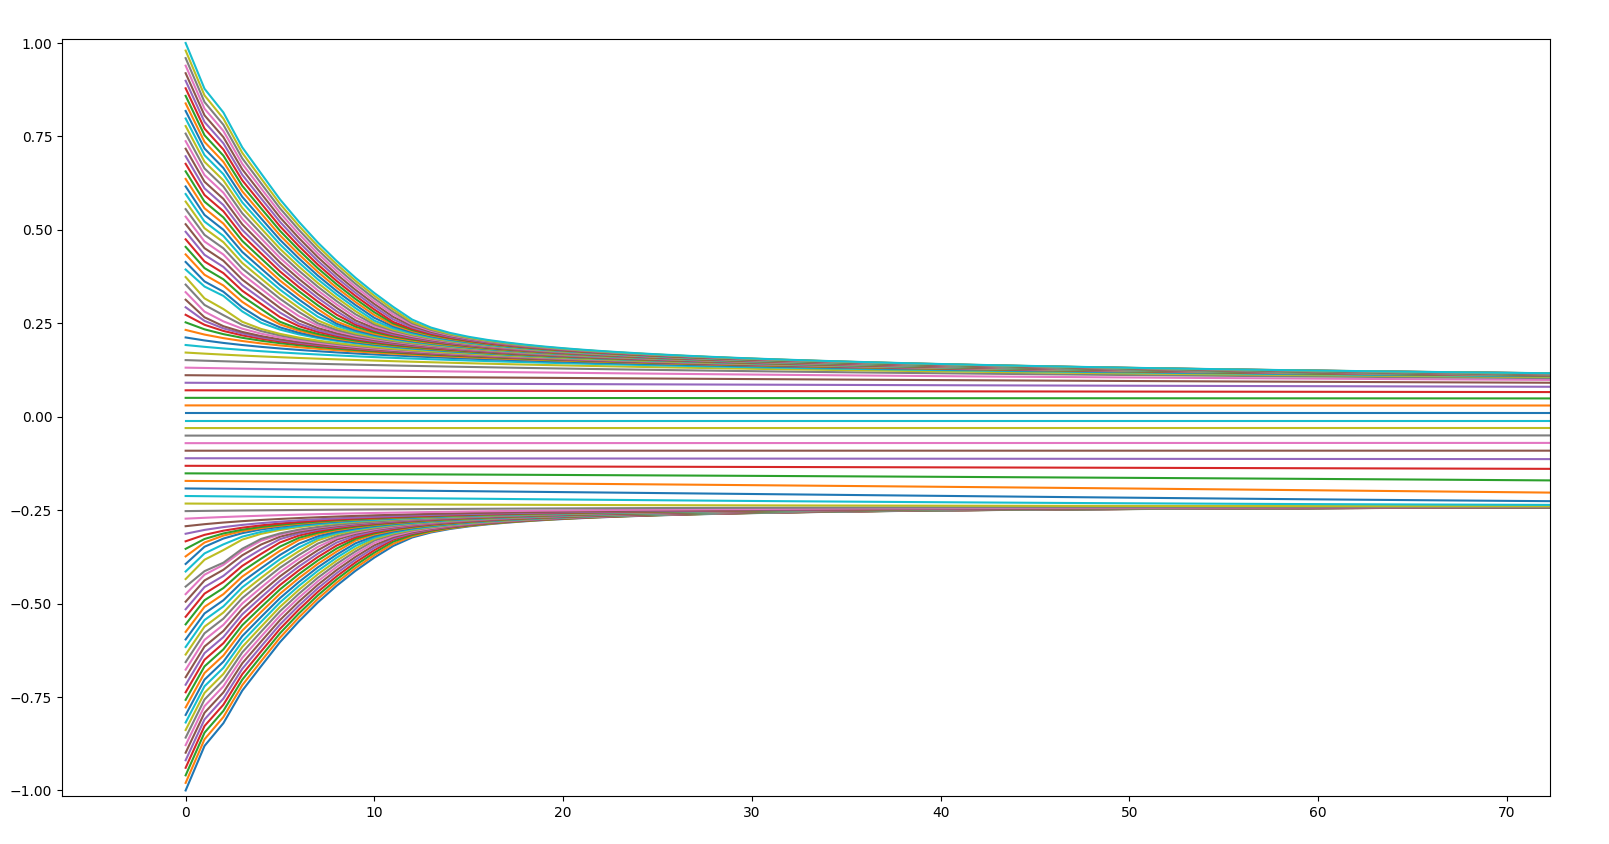
\includegraphics[width = 0.8\textwidth]{Images/p1f1.png}
    \caption{Out to $t = 75$.}
    \label{fig:p1f1}
\end{figure}
\begin{figure}
    \centering
    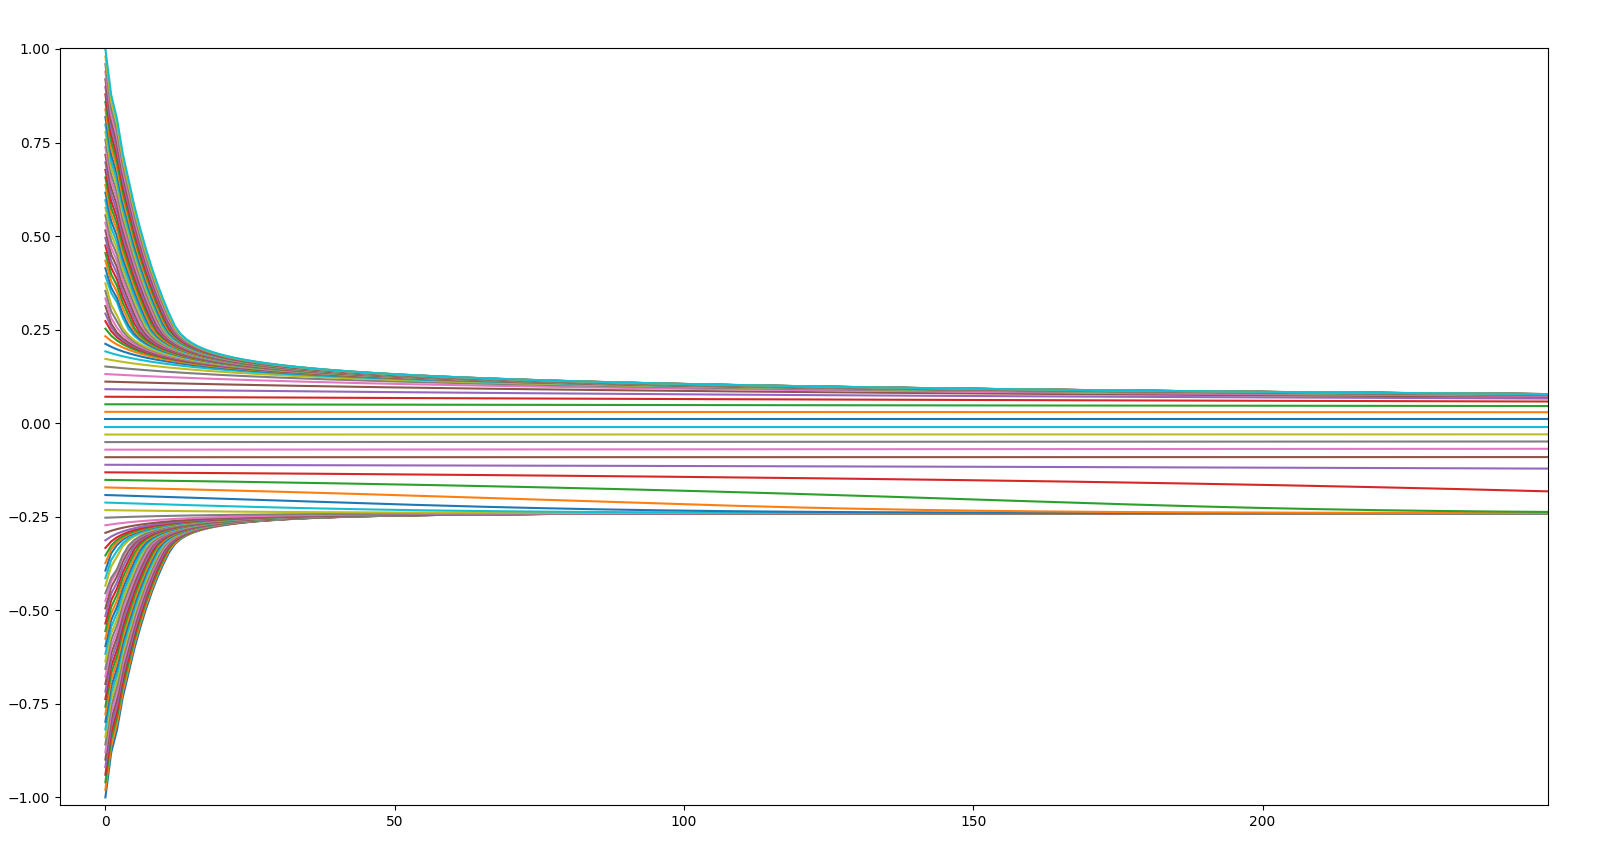
\includegraphics[width = 0.8\textwidth]{Images/p1f2.png}
    \caption{Out to $t = 250$.}
    \label{fig:p1f2}
\end{figure}
\begin{figure}
    \centering
    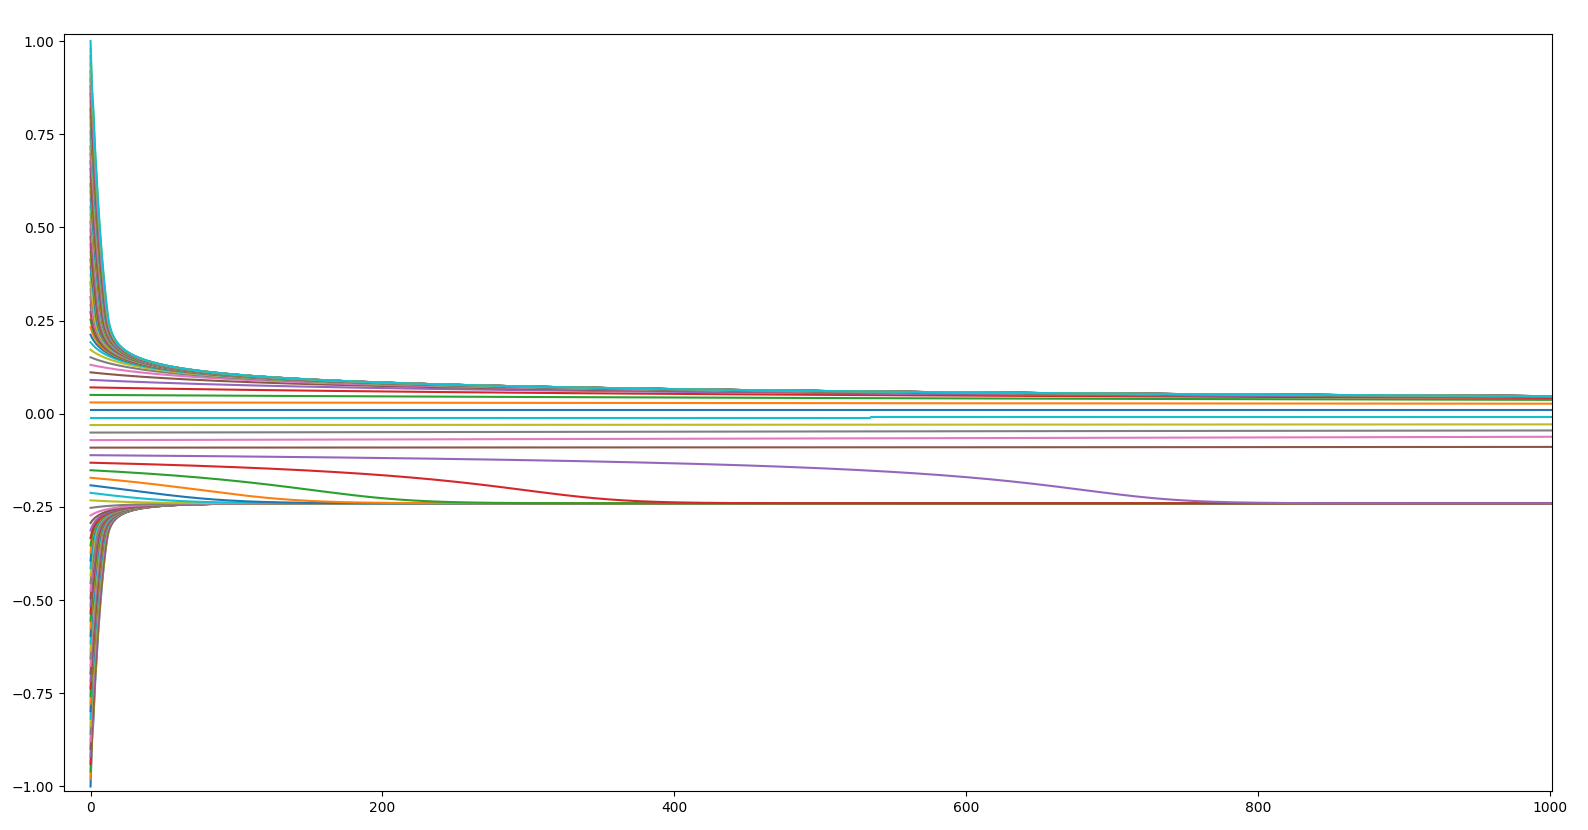
\includegraphics[width = 0.8\textwidth]{Images/p1f3.png}
    \caption{Out to $t = 1000$.}
    \label{fig:p1f3}
\end{figure}
\begin{figure}
    \centering
    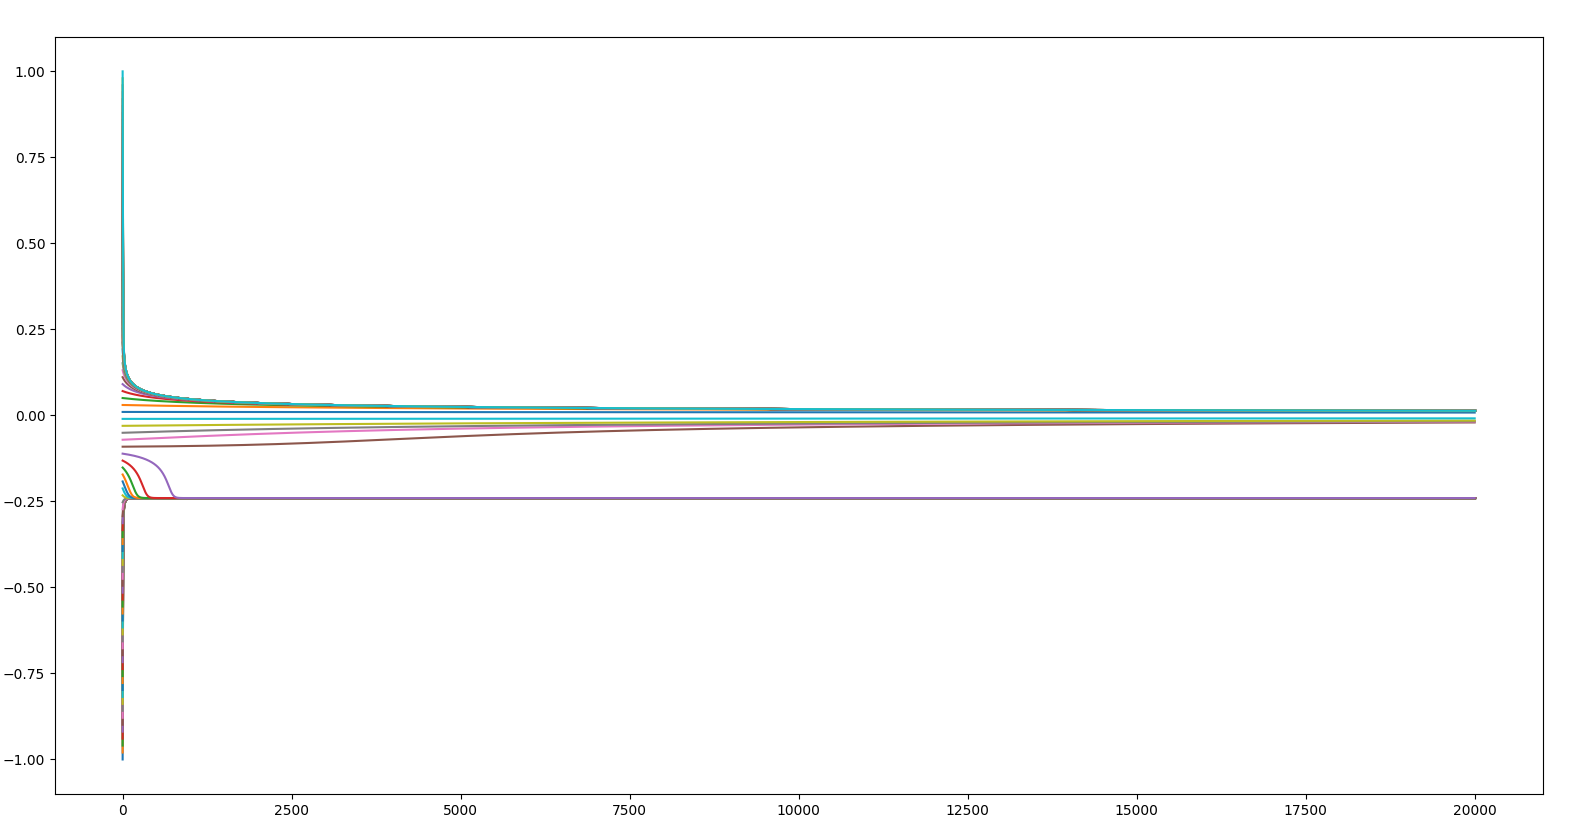
\includegraphics[width = 0.8\textwidth]{Images/p1f4.png}
    \caption{Out to $t = 20000$.}
    \label{fig:p1f4}
\end{figure}

\begin{figure}
    \centering
    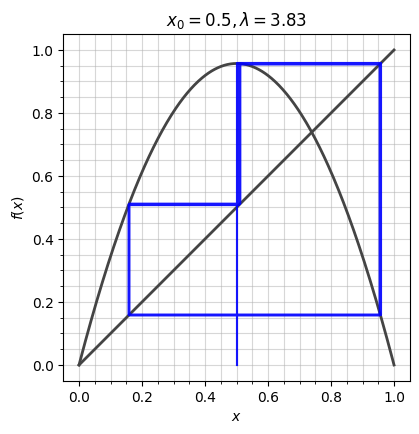
\includegraphics[width = 0.5\textwidth]{Images/cobwek plot.png}
    \caption{Cobweb plot for $x_0 = 0.5, \lm = 3.83$}
    \label{fig:enter-label}
\end{figure}

\clearpage
\newpage
\section{Problem 2}
This is meant to be a simple problem in which you numerically computer a Poincar\'e return map, and use it to determine the Floquet multiplier associated with a limit cycle. Let

\begin{align}
    \xdot &= 2y\nonumber\\
    \ydot &= -2x + \frac{1}{2}(1 - x^2)y\nonumber
\end{align}

Define a surface of section as $\Si = \{(x, y) : x \in [1, 3], y = 0\}$ for your return map, and numerically compute the Poincar\'e return map $P: \si \rightarrow \si $ by computing orbits for initial conditions in $(x_0, 0) \in \si$, and finding the $x$ values where they next return to $\si$, i.e. if the next point is $(x_1, 0) \in \si$, then the map should satisfy $x_1 = P(x_0)$ for each $x_0 \in [1, 3]$. You will find that the map has a fixed point $(P(x^*) = x^*)$, and the $x^*$ value associated with it gives a point $(x^*, 0)$ on a limit cycle for the flow. You can further obtain an estimate of the Floquet multipliers associated with the limit cycle by estimating $\mu = P'(x^*)$. How does this compare with what you obtain from the Monodromy matrix? (According to results proved in Meiss, you should find that the eigenvalues of the Monodromy matrix are exactly $\mu, 1$. You can either prove this for this 2-d example, or compute the Monodromy matrix numerically to confirm the claim.)

\partbreak
\begin{solution}

    I have numerically computed solutions for this system for 40 different in ital conditions within the interval $[1, 3]$, I will provide my plots first, followed by the code. We can see the various solutions in Figure \ref{fig:p2 curves}. It seems that all initial conditions in $\si$ are captured by the equilibrium point at the origin, and follow an approximation of a circle. Figure \ref{fig:p2 return map} reveals the Poincar\'e Return map, which, when compared to the line $y = x$, can be used to approximate the fixed point $x^* = 2$. I have fitted a cubic polynomial to our curve to aid in the estimation of the Floquet Multiplier $\mu$. By what we are given, we can get this estimation via $\mu = P'(x^*)$, where $P$ is our fitted polynomial function. With this, we get that $\mu \approx 0.194$ at $x^* = 2$.\par

    \jump
    To compare this with the values we get for the Monodromy matrix, I will numerically estimate it. For this, we need to numerically solve the linear system, calculate its period, and evaluate the fundamental matrix at that point. I will omit the plot for the linear system, since it's not really important what it looks like, just that we get the period. I estimate the period to be $T = (3.1632 +- 0.0014)$ s. With this, we can get that the Monodromy matrix is
    \begin{align}
        M = \Phi(T) = 
        \begin{bmatrix}
            0.104477621435603 + 0.0299966220466678i, &0\\ 0 &-0.466072701884242 + 0.59323886946441i
        \end{bmatrix}\nonumber\\
    \implies \mu = \{0.104477621435603 + 0.0299966220466678i, -0.466072701884242 + 0.59323886946441i\}
    \end{align}
    These were calculated by the code below. This will result in an incorrect evaluation of the Floquet Multipliers, but the multipliers are the eigenvalues of the monodromy matrix, which is constructed by the eigenvectors of the Linear system multiplied by $e^{\lm_i t}$, then evaluated at the period. This was done, but gave either incorrect results, or is going to be off due to calculation errors. Either way, these two values for the Floquet Multiplier $\mu$ are not equivalent. 
    
    \begin{lstlisting}
    #Finding Monodromy matrix Numerically
    #using Sympy
    t = sp.symbols('t')

    linMat = sp.Matrix([[0, 2], 
                    [-2, 0.5]])

    eigvals, eigvects = linMat.diagonalize()
    Mono = eigvects * sp.diag(sp.exp(eigvals[0] * t), sp.exp(eigvals[1] * t)) * eigvects.inv()
    zeroMat = Mono.subs(t, 0)
    zeroMat_inv = zeroMat.inv()
    res = Mono * zeroMat_inv
    res_at_t = res.subs(t, 3.1632)
    eigenvalues_res = res_at_t.eigenvals()
    
    print(eigenvalues_res)  
    \end{lstlisting}
    
    
    \newpage
    \begin{figure}[ht]
        \centering
        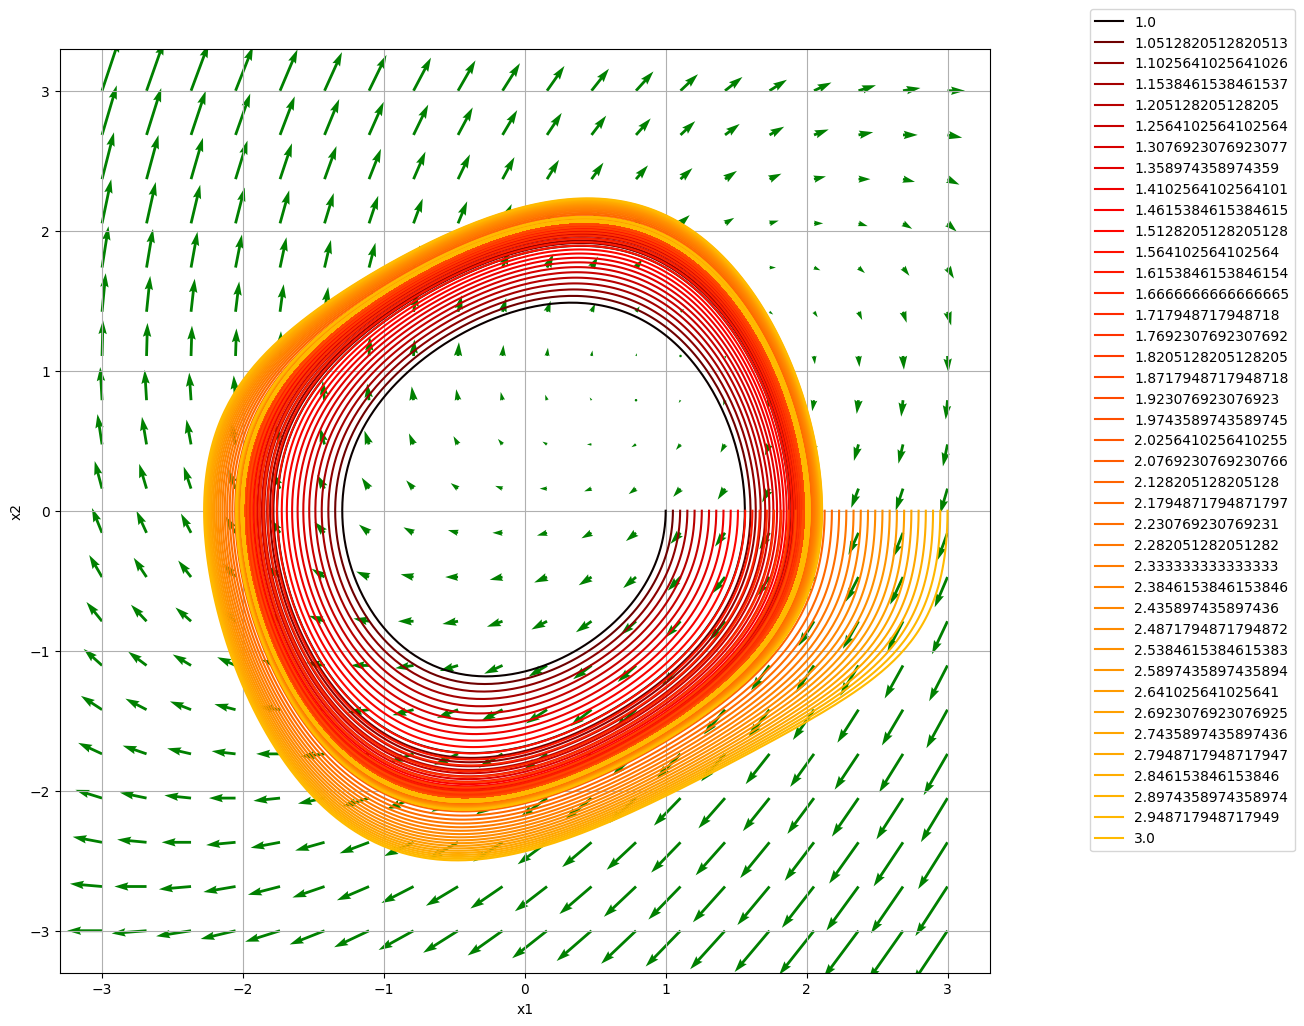
\includegraphics[width = 0.6\textwidth]{Images/problem 2 curves.png}
        \caption{Curves obtained by 40 different initial conditions in $\si$. The vector field for the system is also shown. The image is not tilted, but it does appear to be.}
        \label{fig:p2 curves}
    \end{figure}
    \begin{figure}[!ht]
        \centering
        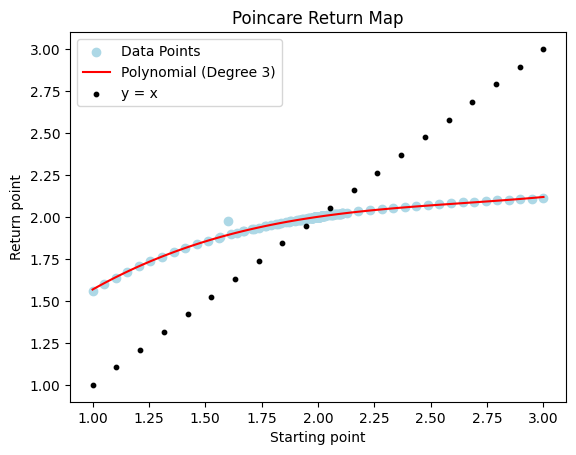
\includegraphics[width = 0.6\textwidth]{Images/Problem 2 return map.png}
        \caption{Poincar\'e Return map for the system. A cubic polynomial has been fit to it to determine the derivative.}
        \label{fig:p2 return map}
    \end{figure}

\newpage
\begin{lstlisting}
#Block to get solutions
import numpy as np
import matplotlib.pyplot as plt
from scipy.integrate import solve_ivp
import matplotlib.cm as cm
import sympy as sp

#System definition
def xdot(y, t):
    x1, x2 = y
    return [2*x2, -2*x1 + 0.5 * (1 - x1**2)*x2]

#Linear System definition
def linxdot(y, t):
    x1, x2 = y
    return [2*x2, -2*x1 + 0.5*x2]

def get_sigma_intersection(x : np.ndarray, y : np.ndarray):
    """
    Returns the array of x values where the solution
    hits the surface defined as the following
    $\Si = \{(x, y) : x \in [1, 3], y = 0\}$
    
    Parameters
    ----------
    x : np.ndarray
        The array of x positions for the solution
    
    y : np.ndarray
        The array of y positions for the solution
    """
    
    eps = 0.001 #Float tolerance
    
    arr = []
    arr.append(x[0])
    for i in range(len(y) - 1):
        if y[i] > eps and y[i+1] < 0:
            arr.append(x[i])
    
    return arr

def get_period(sol):
    """
    Returns the minimal period of the solution
    """
    x0 = sol.y[0][0]
    x, y = sol.y
    
    for i in range(len(x)):
        if y[i] > 0 and y[i+1] < 0:
            return sol.t[i]    

#define time range
timespan = (0., 500.)
init = 40 #number of initial conditions

#initial conditions
x0s = np.linspace(1, 3, init)
y0 = 0.0
i = 0
max_len = 0

colors = np.linspace(0, 1 / max(max(x0s), 1), init)
fig, axs = plt.subplots(1, 1, figsize =(12, 12))

for x0 in x0s:
    initial_conditions = [x0, y0]
    #Getting numerical Solution

    sol = solve_ivp(lambda t, y: xdot(y, t), t_span=timespan,
                    y0=initial_conditions, max_step = 0.01)
    #Picking coords of solution
    x, y = sol.y
    axs.plot(x, y, color = cm.hot(min(colors[i]**0.4, 0.7)), label = x0)
    
    i+=1
    
    
#resizing xpts array
xpts = xpts[:, :max_len]

bounds = 3
#Vector Field meshes
xvect, yvect = np.meshgrid(np.linspace(-bounds, bounds, 20),
                           np.linspace(-bounds, bounds, 20))

#Update vector fields
uvect = -1 + yvect
vvect = yvect - xvect

# Plotting Vector Field
axs.quiver(xvect, yvect, uvect, vvect, color='g')

axs.grid(True)

axs.set_xlabel("x1")
axs.set_ylabel("x2")
axs.legend(bbox_to_anchor=(1.1, 1.05))

# Show plot with grid
plt.show()
\end{lstlisting}

\begin{lstlisting}
#Block for Poincare Return map
ret_map = []
for curve in xpts:
    for i in range(len(curve[:7])):
        ret_map.append((curve[i], curve[i+1]))
ret_map = np.array(ret_map)

#sorting points 
sorted_indices = np.argsort(ret_map[:, 0])
sorted_data = ret_map[sorted_indices]

#Obtaining a Polynomial fot to the curve
coefficients = np.polyfit(sorted_data[:, 0], sorted_data[:, 1], 3)
poly_function = np.poly1d(coefficients)
x_curve = np.linspace(min(sorted_data[:, 0]), max(sorted_data[:, 0]), 100)
y_curve = poly_function(x_curve)

#Plotting
plt.scatter(sorted_data[:, 0], sorted_data[:, 1], label='Data Points', c='lightblue')
plt.plot(x_curve, y_curve, label=f'Polynomial (Degree {3})', color='red')
plt.xlabel('Starting point')
plt.ylabel('Return point')
plt.scatter(np.linspace(1, 3, 20), np.linspace(1, 3, 20), label = "y = x", color = 'k', s=10)
plt.title("Poincare Return Map")
plt.legend()
\end{lstlisting}

\begin{lstlisting}
#Estimating period of linear system and plotting
#define time range
timespan = (0., 50.)
init = 4 #number of initial conditions

#initial conditions
x0s = np.linspace(1, 3, init)
y0 = 0.0
i = 0
max_len = 0
Periods = np.zeros((init, 1)) #Minimal periods for initial conditions
colors = np.linspace(0, 1 / max(max(x0s), 1), init)
fig, axs = plt.subplots(1, 1, figsize =(12, 12))

for x0 in x0s:
    initial_conditions = [x0, y0]
#Getting numerical Solution

    sol = solve_ivp(lambda t, y: linxdot(y, t), t_span=timespan,
                    y0=initial_conditions, max_step = 0.01)
    #Picking coords of solution
    x, y = sol.y
    axs.plot(x, y, color = cm.hot(min(colors[i]**0.4, 0.7)), label = x0)
    period = get_period(sol)
    Periods[i] = period
    i+=1
    
    
#resizing xpts array
xpts = xpts[:, :max_len]

axs.grid(True)

axs.set_xlabel("x1")
axs.set_ylabel("x2")
axs.legend(bbox_to_anchor=(1.1, 1.05))

print("Estimation of the Period: {:.4f} += {:.4f}".format(Periods.mean(), Periods.std()))
# Show plot with grid
plt.show()
\end{lstlisting}
\end{solution}

\clearpage

\newpage
\section{Problem 3}
Now consider the R\"ossler dynamical system in $\R^3$:
\begin{gather*}
    \xdot = -y - z\\
    \ydot = x+ay\\
    \dot{z} = b + z(x - c)
\end{gather*}
with $a = b = 0.2$.
\subsection{Problem 3, part a}
Let $c = 2.5$ and find, by numerical solution of the equations, a stable limit cycle. For this next, part, you will need to know a point $(x_0, y_0, z_0)$ on the limit cycle to good precision, and also the period $T$ for the limit cycle to good precision.
\partbreak
\begin{solution}

    The initial conditions I found to give a good band were $(x_0, y_0, x_0) = (4.7, -1.1430, 0.85)$. With this I found the period to be roughly $T = 63.25$. The plot for this system, as well as the code to plot it and compute its period is given below.

    \begin{figure}[h]
        \centering
        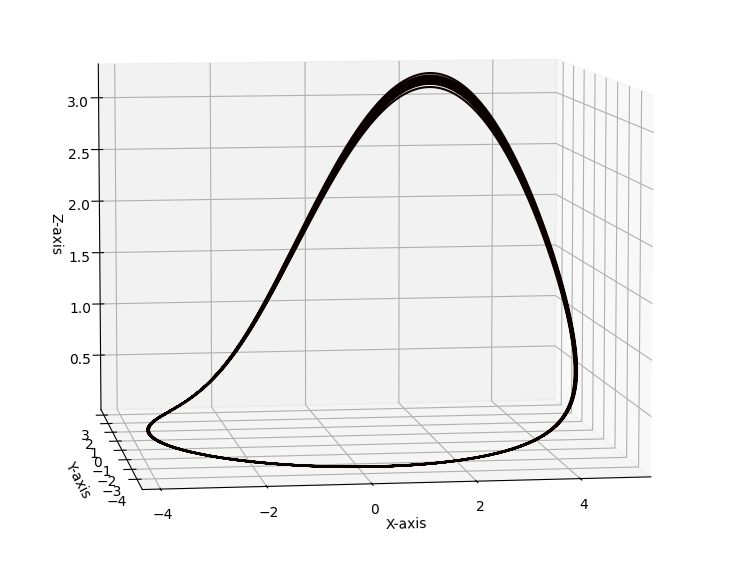
\includegraphics[width = 0.5\textwidth]{Images/p3im.png}
        \caption{R\"ossler System for given initial conditions. The period is given is $T\approx 63.25$.}
        \label{fig:p3 system}
    \end{figure}

\newpage
\begin{lstlisting}
import numpy as np
import matplotlib.pyplot as plt
from scipy.integrate import solve_ivp
import matplotlib.cm as cm
import math
from mpl_toolkits.mplot3d import Axes3D
%matplotlib qt

#System definition
def xdot(y, t, a, b, c):
    x1, x2, x3 = y
    return [ - x2 - x3,
               x1 + a * x2,
               b + x3 * (x1 - c)]

def get_period(sol):
    """
    Gets the Minimum period of the solution
    """
    x0, y0, z0 = sol.y[:, 0]
    init = np.array([x0, y0, z0])
    x, y, z = sol.y
    dist = np.zeros(x.shape[0])
    for i in range(len(dist)):
        ipoint = np.array([x[i], y[i], z[i]])
        dist[i] = math.dist(init, ipoint)

    dist_arr = []
    for i in range(len(dist[2:])):
        if dist[i-1] > dist[i] and dist[i+1] > dist[i] and dist[i] != 0:
            dist_arr.append((sol.t[i], dist[i]))
    
    sorted_tuples = sorted(dist_arr, key=lambda x: (x[1], x[0]))
    
    return sorted_tuples[0][0]

#define time range
timespan = (0., 100.)
init = 1 #number of initial conditions

#Paramters
a = 0.2
b = 0.2

#initial conditions
x0 = 4.7
y0 = -1.1430
z0 = 0.85
i = 0

colors = np.linspace(0, 1 / 1, 1)
fig = plt.figure()
axs = fig.add_subplot(111, projection='3d')

initial_conditions = [x0, y0, z0]

c = 2.5
sol = solve_ivp(lambda t, y, a, b, c: xdot(y, t, a, b, c), t_span=timespan, y0=initial_conditions, max_step=0.01, args=(a, b, c))
#Picking coords of solution
x, y, z = sol.y
axs.plot(x, y, z, color = cm.hot(min(colors[i]**0.4, 0.7)), label = x0)
axs.view_init(elev=20, azim=45) 
axs.set_xlabel('X-axis')
axs.set_ylabel('Y-axis')
axs.set_zlabel('Z-axis')

print(f'Period: {get_period(sol)}')
# Show the plot
plt.show()

\end{lstlisting}
\end{solution}

\newpage
\subsection{Problem 3, part b}
Linearize the equations about the limit cycle and compute the Monodromy matrix $M$, together with its eigenvalues $\mu$, which are called Floquet multipliers. Meiss describes how to do this numerically using the point $(x_0, y_0, z_0)$ as an initial condition for the limit cycle $\gamma(t) = \gamma(T)$. Find the eigenvector associated with the eigenvalue $\mu = 1$. Show that it points in a direction that is is along the limit cycle at $(x_0, y_0, z_0)$.
\partbreak
\begin{solution}

    To linearize the system, we denote our chosen $(x_0, y_0, z_0)$ from part a as such. Then, we take the Jacobian of our system, the evaluate it on our limit cycle. I will chose to evaluate the periodic cycle at my chosen initial conditions. Thus, 

    \alignbreak
    \begin{align}
        f &= (-y - z, x + ay, b + z(x - c)) &\text{(Our system.)}\nonumber\\
        \implies Df(\gamma(t)) &= \begin{bmatrix}0 &-1 &-1\\ 1 &a &0\\ z &0 &x - c\end{bmatrix} &\text{(Taking Jacobian.)}\nonumber\\
        \implies Df(\gamma(0)) = Df(\textbf{x}_0) &=  \begin{bmatrix}0 &-1 &-1\\ 1 &a &0\\ z_0 &0 &x_0 - c\end{bmatrix} &\text{(Evaluating on limit cycle.)}\nonumber
    \end{align}
    \alignbreak
    Note This was entirely independent on the stated values of the initial conditions. when plugging in $(x_0, y_0, x_0) = (4.7, -1.1430, 0.85)$, we get that the magnitudes of the eigenvalues are $(1.13053, 1.13053, 1.8543)$, which is admittedly not what we wanted to see. 
\end{solution}

\newpage
\subsection{Problem 3, part c}
Starting with $c = 2.5$, find a stable limit cycle and investigate its stability properties
as you gradually increase $c$. You should find that it loses stability when an eigenvalue of the
Monodromy matrix crosses the unit circle at $\mu = -1$. What is the $c$ value associated with this? What happens to the limit cycle for $c$ increasing further?
\partbreak
\begin{solution}

    Even though something appears to be incorrect in the previous part, I tried investigating what happened when we increase for various values of $c$. You can see how the eigenvalues change in the given plot below. It appears that when the solely real eigenvalue breaches -1, at roughly $c = 5.3$, we get see the plot take on a notably different shape, and the period somehow gets smaller, $T \approx 17.4099$.
\end{solution}

\begin{figure}[h]
    \centering
    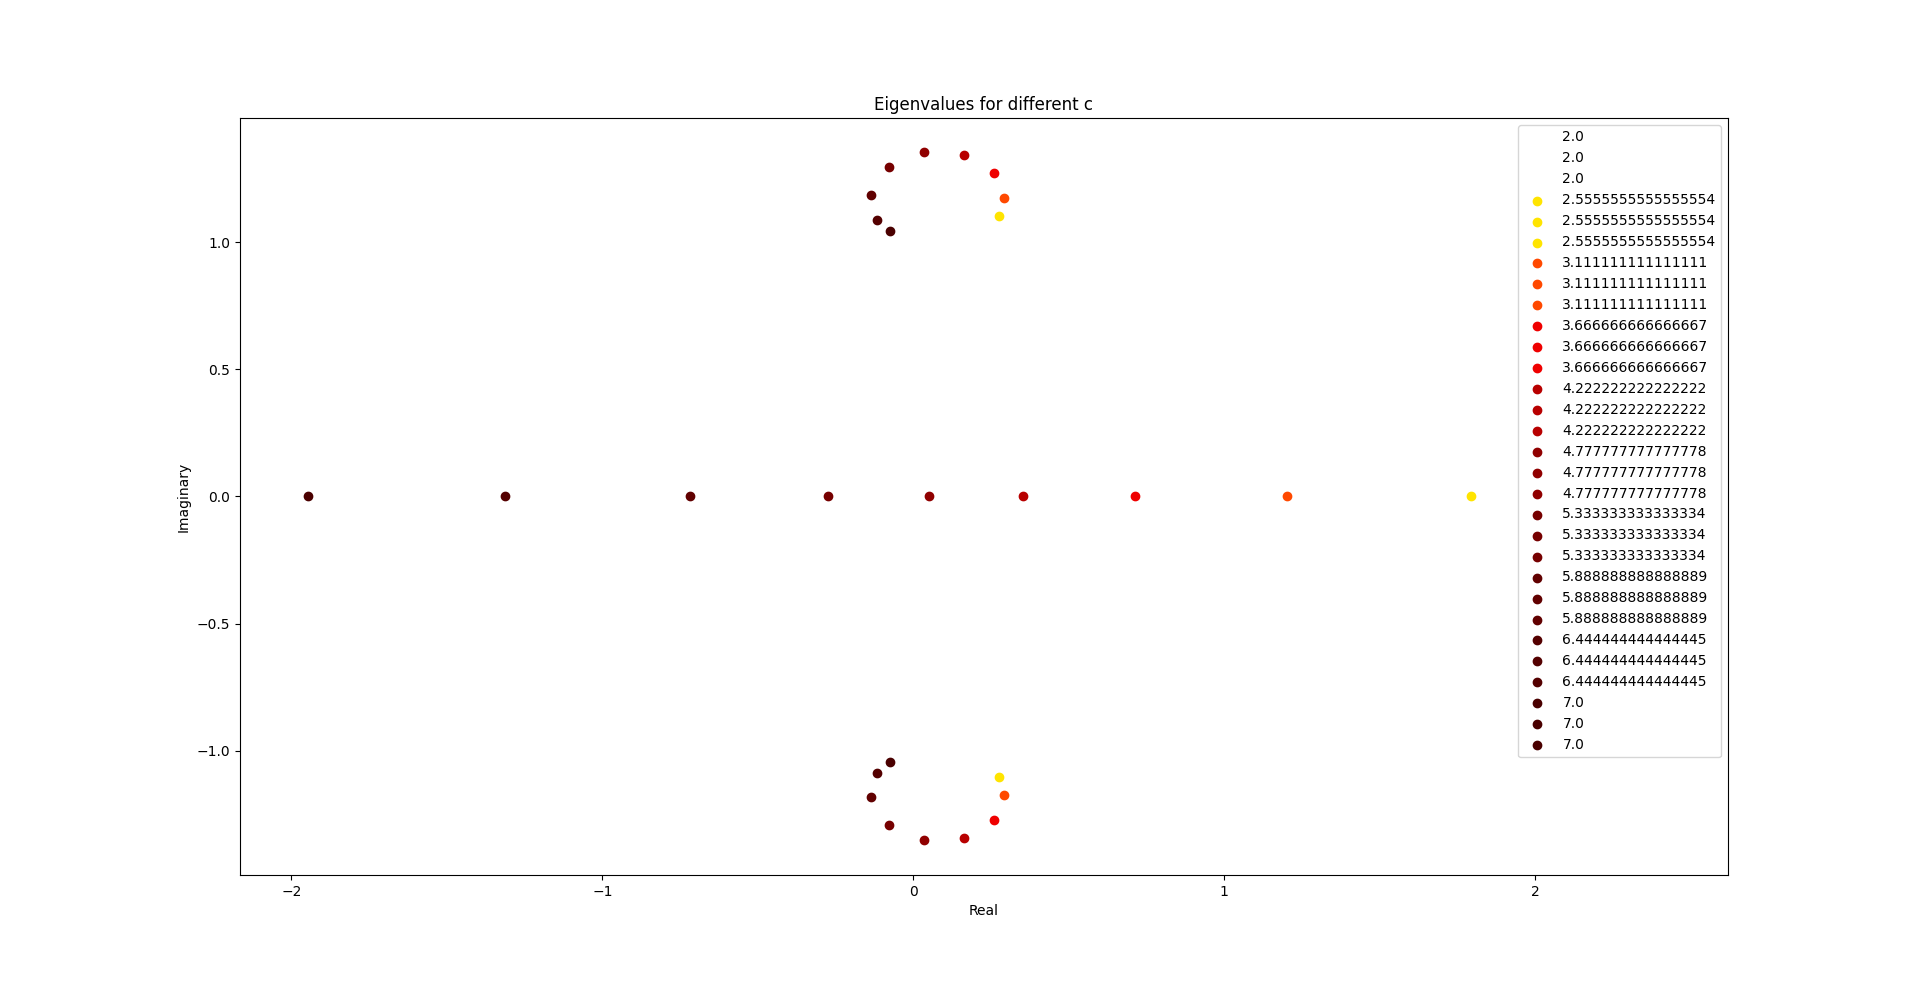
\includegraphics[width = 0.8\textwidth]{Images/eigvals plot.png}
    \caption{Eigenvalues for various $c$. Note there is one eigenvalue which is entirely positive, and two others that pivot around a certain point in the complex plane. Apologies for the terrible legend.}
    \label{fig:p3shit}
\end{figure}

\begin{figure}
    \centering
    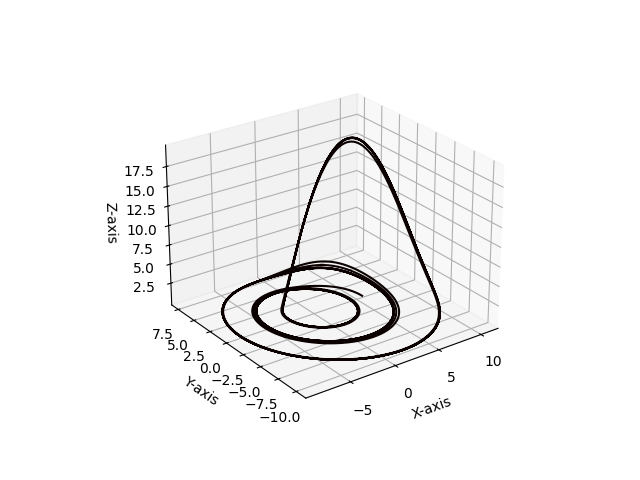
\includegraphics{Images/p3 bullshit.png}
    \caption{The R\"ossler system for $c = 5.3$. Note the period has decreased to roughly 17.4, and the system seems to experience ``triple period doubling".}
    \label{fig:p3 newplot}
\end{figure}
\newpage
\section{Problem 4}
Consider the Lorenz equations
\begin{align}
    \xdot &= \sigma(y - x) \nonumber\\
    \ydot &= rx - y - xz \nonumber\\
    \dot{z} &= xy - bz, \nonumber    
\end{align}
where $r, b, \sigma$ are positive constants and $(x, y, z)\in \R^3$.

\subsection{Problem 4, part a}
Show that the origin is the only fixed point for $r \in (0, 1]$, and that the following is a strong Lyapunov function for it for $r < 1$:
\[
L = \frac{1}{2}\Big( \frac{x^2}{\sigma} + y^2 + z^2\Big)
\]
\partbreak
\begin{solution}

    By plugging in $(x, y, z) = (0, 0, 0)$ into the Lorenz equations, we see that the origin is a fixed point. Next we want to show it is the only fixed point for $r \in (0, 1]$. Suppose this were false, then there would be some $\textbf{x} = (x_1, x_2, x_3)$ such that $f(\textbf{x}) = \textbf{x}$, where $f$ is the right hand side of the Lorenz equations above. Then, we get the following system of equations

\begin{align}
    \sigma(x_2 - x_1) &= x_1 &(1)\nonumber\\
    rx_1 - x_2 - x_1x_3 &= x_2 &(2)\nonumber\\
    x_1x_2 - bx_3 &= x_3 &(3) \nonumber
\end{align}

Note that by observation, if any combination of $x_1, x_2, x_3 = 0$, then all are zero. More importantly, if any coordinate of our proposed fixed point is zero, then $\textbf{x} = 0$. I will demonstrate this below.\par

\jump
If $x_1 = 0$, then by (3), $x_3(1 + b) = 0$. Since we are given $b$ is a positive constant, $x_3 = 0$. Then by (1), $x_2 = 0$. So if $x_1 = 0, \textbf{x} = 0$. Similarly, if $x_2 = 0$, then by (3), $x_3(1 + b) = 0$, so $x_3 = 0$. Also, by (2), $rx_1 = 0$. Since $r \in (0, 1]$, then $x_1 = 0$, thus $\textbf{x} = 0$ when $x_2 = 0$. Finally, if $x_3 = 0$, then by (3), $x_1x_2 = 0$. Thus $x_1$ or $x_2$ = 0. We already showed if $x_1$ = 0, then $x_2 = 0$, as well as is converse. Thus $\textbf{x} = 0$ when $x_3 = 0$. Therefore if any coordinate of our proposed fixed point is zero, then our fixed point is zero. We want to show that our proposed fixed point is unique from the origin, so we can omit the cases where any coordinate equals zero in the below steps:

\alignbreak
\begin{align}
    x_1 &= \frac{\sigma}{1 + \sigma} x_2  &\text{(From (1).)}\nonumber\\
    0 &= \frac{r\sigma}{1 + \sigma}x_2 - x_2 - \frac{1}{1 + \sigma}x_2x_3 - x_2 &\text{((1) $\rightarrow$ (2).)}\nonumber\\
    \implies 0 &= x_2(\frac{r\sigma}{1 + \sigma} - 2 - \frac{\sigma}{1 + \sigma}x_3) &\text{(Rearranging.)}\nonumber\\
    \implies 0 &= \frac{r\sigma}{1 + \sigma} - 2 - \frac{\sigma}{1 + \sigma}x_3&\text{(Should hold for all $x_2$.)}\nonumber\\
    \implies x_3 &= r - 2 - \frac{2}{\sigma} &\text{(Simplifying.)}\nonumber\\
    3) : \ x_1x_2 &- b(r - 2 - \frac{2}{\sigma}) = r - 2 - \frac{2}{\sigma} &\text{(Plugging in $x_3$ to (3).)}\nonumber\\
    \implies x_1x_2 &= (1 + b)(r - 2 - \frac{2}{\sigma}) &\text{(Simplifying.)}\nonumber\\
    1) : \ x_1x_2 &= \sigma x_2^2 - \sigma x_1x_2 &\text{(Multiplying (1) by $x_2 \neq 0$.)}\nonumber\\
    x_2^2 &= \frac{1+\sigma}{\sigma} x_1x_2 &\text{(Rearranging.)}\nonumber\\
    \implies x_2 &= \sqrt{\Big(\frac{r\sigma - 2(1 + \sigma)}{\sigma}\Big)(1 + b)\Big(\frac{1+\sigma}{\sigma}\Big)} &\text{(Solving for $x_2$.)}\nonumber
\end{align}
\alignbreak

Note that we want only real values for $x_2$, so each term under the square root should be positive. Each term above is guaranteed to be positive, except for the first, imposing $r\sigma - 2(1 + \sigma) \geq 0$. Rearranging for $r$, we get
\[
r \geq \frac{2}{\sigma} + 2
\]

Note that since $\sigma \geq 0$, then $\frac{2}{\sigma} \geq 0$. Thus $r$ has to be \textit{at least} 2, which is a contradiction, since we are restricting $r \in (0, 1]$. Thus there are no other fixed points of the Lorenz system aside from the origin for $r \in (0, 1]$.\par

\newpage
Next we want to show that the given Lyapunov function
\[
L = \frac{1}{2}\Big( \frac{x^2}{\sigma} + y^2 + z^2\Big)
\]

is a strong Lyapunov function for the Lorenz system. Note this is equivalent to showing $\frac{dL}{dt} < 0$ for all $t > 0$. Thus, the following steps hold:
\alignbreak
\begin{align}
    \frac{dL}{dt} &= \frac{1}{2}\Big( \frac{2}{\sigma}x\xdot + 2y\ydot + 2z\dot{z} \Big)&\text{(Differentiation.)}\nonumber\\
    &= (y - x)x + y(rx - y - xa) + z(xy - bz) &\text{(Plugging in Lorenz System.)}\nonumber\\
    &= (1 + r) xy - x^2 - y^2 - bz^2 &\text{(Simplifying.)}\nonumber\\
    &< 2xy - x^2 - y^2 - bz^2 &\text{(Restriction on $r$.)}\nonumber\\
    &= -(x - y)^2 - bz^2 &\text{(Difference of squares.)}\nonumber\\
    &= -((x - y)^2 + bz^2) &\text{(Grouping.)}\nonumber\\
    &\leq 0 &\text{(argument inside is positive.)}\nonumber\\
\implies \frac{dL}{dt} &< 0 &\text{(Summary.)}\nonumber
\end{align}
\alignbreak
\end{solution}

\newpage
\subsection{Problem 4, part b}
Show that $L$ is only a weak Lyapunov function if $r = 1$, but that you can use LaSalle's Invariance Principle to prove that the origin is asymptotically stable for $r = 1$ as well as for $r < 1$. Note that you did not have to restrict any of this to a particular neighborhood $U$ of the origin. The origin is globally attracting for the Lorenz equations when $r \in (0, 1]$.

\partbreak
\begin{solution}

    For the sake of completeness, I will include LaSalle's Invariance Principle.
    \begin{quote}
        \underline{\textbf{LaSalle's Invariance Principle:}} \\
        Suppose $x^*$ is a fixed point of the equilibrium of $\ph_t(x)$ and $L$ is a weak Lyapunov function of $x^*$ on some compact forward invariant neighborhood $U$ of $x^*$. Let $Z = \{x \in U : dL/dt = 0\}$. If $\{x^*\}$ is the largest forward invariant subset of $Z$, then $x^*$ is asymptotically stable and attracts every point in $U$.
    \end{quote}

    Note the only way we could have gotten a strong Lyapunov function on the previous part was on the restriction of $r$, i.e., $1 + r < 2$. Since $r = 1$, this bound becomes an equality, which implies that our Lyapunov function is now only weak. \par

    \jump
    Since the Lorenz system is globally attracted to the origin for $r \in (0, 1]$, we can just take the neighborhood $U$ to be the whole range of the system, thus making $U$ compact and forward invariant. Next, we just want to show that $\{(0, 0, 0)\}$ is the largest forward invariant subset of $Z$. Note that we found the derivative of our Lyapunov function in the previous part, 
    \[
    \frac{dL}{dt} = -((x - y)^2 + bx^2),
    \]
    where I implicitly took the restriction that $r = 1$. The function inside the outer parenthesis is a sum of two squares, thus positive. It only has one real root, namely at $x = y = z = 0$, thus $Z = \{(0, 0, 0)\}$, meaning aside from the empty set, the origin is the only point contained in $Z$. It is also a forward invariant subset, since the origin is a stable point of the Lorenz system for $r \in (0, 1]$. Thus by LaSalle's Invariance Principle, $x^* = (0, 0, 0)$ is asymptotically stable and attracts every point in our solution space $U$ for $r \in (0, 1]$.
\end{solution}

\newpage
\section{Problem 9}
An asymptotically stable linear system always has a Lyapunov function of the form $L = \textbf{x}^TS\textbf{x}.$

\subsection{Problem 9, part a}
Show that when all the eigenvalues of $A$ have negative real parts, then the        Lyapunov equation" has the unique, positive definite, symmetric solution
\[
S = \int_0^\infty e^{\tau A^T}e^{\tau A}d\tau
\]
\partbreak
\begin{solution}

    Taking inspiration from the hint given, let us pre- and post- multiply the Lyapunov Equation by $e^{tA^T}$ and $e^{tA}$ respectively. 

    \[
    \implies e^{tA^T}(A^TS + SA)e^{tA} = -e^{tA^T}e^{tA}
    \]

    Note that the left hand side appears to be a total time derivative. With careful inspection, we can recover the function
    \[
    \frac{d}{dt}\Big[ e^{tA^T}Se^{tA} \Big] = -e^{tA^T}e^{tA}.
    \]

    Thus integrating both sides, and applying the Fundamental Theorem of Calculus to the left hand side gives
    \[
    \lim_{\tau \rightarrow \infty} \Big[ e^{\tau A^T}Se^{\tau A}\Big] - \lim_{t \rightarrow 0} \Big[ e^{\tau A^T}Se^{\tau A}\Big] = -\int_0^\infty e^{\tau A^T}e^{\tau A} d\tau
    \]

    The limit approaching zero is straightforward and does not depend on the eigenvalues of $A$, so the second limit equals $S$. The first limit however, relies on the real parts of the eigenvalues of $A$ being negative. This limit will equal zero, as can be recovered by eigenvalue decomposition of $A$, then applying the exponential. Thus we can write the following
    \[
    S = \int_0^\infty e^{\tau A^T}e^{\tau A} d\tau
    \]

    This is the equation we wanted to show, we just need to check the following:
    \begin{enumerate}
        \item \underline{Uniqueness:}

        If there is an $S'$ with $S \neq S'$ such that $S' = \int_0^\infty e^{\tau A^T}e^{\tau A} d\tau$, then $S - S' = \int_0^\infty e^{\tau A^T}e^{\tau A} - e^{\tau A^T}e^{\tau A} d\tau = \int_0^\infty 0 d\tau = 0$. Thus $S = S'$.
        \item \underline{Positive Definiteness:}

        We just need to show $\textbf{x}^TS\textbf{x} > 0$ for all $\textbf{x} \neq 0$.
        \[
        \textbf{x}^TS\textbf{x} = \int_0^\infty \textbf{x}^T e^{\tau A^T}e^{\tau A} d\tau\textbf{x} =  \int_0^\infty \norm{e^{tA}\textbf{x}}^2 d\tau > 0
        \]
        Note we can say the integral is strictly positive since the norm function is itself strictly posiitve when its argument is nonzero.
        \item \underline{Symmetry:}

        This relies on the fact that $(e^{A})^T = e^{A^T}$. With this, we get

        \[
        S^T = \Big[ \int_0^\infty e^{\tau A^T}e^{\tau A} d\tau\Big]^T = \int_0^\infty (e^{\tau A^T}e^{\tau A})^T d\tau = \int_0^\infty e^{\tau A^T}e^{\tau A} d\tau = S
        \]
    \end{enumerate}
\end{solution}

\subsection{Problem 9, part b}
Compute S for the matrix $A = \begin{pmatrix}-2 &1\\ 0 &-2\end{pmatrix}$ and demonstrate explicitly that $dL/dt > 0$.
\partbreak
\begin{solution}

    Note that $A$ can be written as a scalar times the identity matrix plus a nilpotent matrix of degree 2, meaning
    \[
    A = \begin{bmatrix}-2 &0\\ 0 &-2\end{bmatrix} + \begin{bmatrix}0 &1\\ 0 &0\end{bmatrix}
    \]

    When exponentiating, we can then break these up into
    \[
    e^{tA} = e^{-2t\id} * e^N.
    \]

    When taking the matrix exponent of a diagonal matrix, the result is just the exponentiated diagonal elements. Note that by the definition of the matrix exponent, the only terms that survive in the case of the nilpotent matrix is when $k = 0, 1$. Thus,
    \begin{align}
            e^{tA} &= \begin{bmatrix}e^{-2t} &0\\0 &e^{-2t}\end{bmatrix}\Bigg( \begin{bmatrix}1 &0 \\0 &1\end{bmatrix} + \begin{bmatrix}0 &t\\ 0 &0\end{bmatrix}\Bigg)\nonumber\\
            &= \begin{bmatrix}e^{-2t} &0\\0 &e^{-2t}\end{bmatrix}\begin{bmatrix}1 &t \\0 &1\end{bmatrix}\nonumber\\
            &= \begin{bmatrix}e^{-2t} &te^{-2t}\\ 0 &e^{-2t}\end{bmatrix}\nonumber
    \end{align}
    We can note that $e^{tA^T}$ is just this matrix, just transposed, as noted above. Therefore, the following can be done:

    \newpage
    \alignbreak
    \begin{align}
        S &= \int_0^\infty \begin{bmatrix}e^{-2t} &0\\ te^{-2t} &e^{-2t}\end{bmatrix}\begin{bmatrix}e^{-2t} &te^{-2t}\\ 0 &e^{-2t}\end{bmatrix}dt&\text{(Explained above.)} \nonumber\\
        &= \int_0^\infty \begin{bmatrix}e^{-4t} &te^{-4t} \\ te^{-4t} &t^2e^{-4t} + e^{-2t}\end{bmatrix} dt &\text{(Matrix multiplication.)}\nonumber\\
        &=  \begin{bmatrix}\int_0^\infty e^{-4t} dt & \int_0^\infty te^{-4t} dt \\ \int_0^\infty te^{-4t} dt & \int_0^\infty t^2e^{-4t} + e^{-4t}dt\end{bmatrix} &\text{(Integration of a matrix.)}\nonumber\\
        &= \begin{bmatrix}\frac{1}{4} &\frac{1}{16}\\\frac{1}{16} &\frac{9}{32}\end{bmatrix} &\text{(Integration.)}\nonumber
    \end{align}
    \alignbreak
    Note that I used Wolfram Alpha to calculate these integrals for me. In order to show that $dL/dt < 0$, we just need to show this $S$ works in the Lyapunov equation. If so, then $dL/dt = -\norm{\textbf{x}}^2 < 0$ for nonzero $\textbf{x}$.
    \alignbreak
    \begin{align}
        A^TS + SA &= \begin{bmatrix}-2 &0 \\1 &-2\end{bmatrix} \begin{bmatrix}\frac{1}{4} &\frac{1}{16}\\\frac{1}{16} &\frac{9}{32}\end{bmatrix} + \begin{bmatrix}\frac{1}{4} &\frac{1}{16}\\\frac{1}{16} &\frac{9}{32}\end{bmatrix}\begin{bmatrix}-2 &1 \\0 &-2\end{bmatrix}\nonumber\\
        &= \begin{bmatrix}-\frac{1}{2} &-\frac{1}{8}\\ \frac{1}{8} & -\frac{1}{2}\end{bmatrix} + \begin{bmatrix}-\frac{1}{2} &\frac{1}{8}\\ -\frac{1}{8} & -\frac{1}{2}\end{bmatrix}\nonumber\\
        &= \begin{bmatrix}-1 &0 \\0 &-1\end{bmatrix}\nonumber\\
        &= -\id\nonumber
    \end{align}
    \alignbreak
\end{solution}

\newpage
\section{Problem 10}
The Lyapunov function defined in the previous problem also works when nonlinear terms are added to the ODE. Consider the system $\xdot = Ax + g(x)$, where $g(x) = o(x)$ and $A$ is a matrix whose eigenvalues have negative real parts. Show that there is a neighborhood $U$ of the origin for which the function $L = \textbf{x}^TS\textbf{x}$, where $S$ is given in the previous problem, is a strong Lyapunov function.
\partbreak
\begin{solution}

    We must show the two conditions necessary for $L$ to be a strong Lyapunov function. 
    \begin{enumerate}
        \item \underline{$L(\textbf{x}^*) = 0$ for $x^* = 0$.}
        
        Note it was shown in the previous problem that $S$, when written as such, is positive definite. Thus $\textbf{x}^TS\textbf{x}$ is positive for $\textbf{x}\neq 0$. Thus, only when $\textbf{x}^* = \textbf{0}$ do we have that $L = 0$. 

        \item \underline{$dL/dt < 0$}:

        Note that by definition, since $g(x) = o(x)$, for any $\ep > 0$ we are guaranteed a $\delta > 0$ such that when $\norm{x} \leq \delta, \norm{g(x)} \leq \ep$. Therefore, the following steps can be taken:
        \vspace{-5mm}
        \alignbreak
        \vspace{-5mm}
        \begin{align}
            \frac{dL}{dt} &= \dot{\textbf{x}}^T S \textbf{x} + \textbf{x}^TS\dot{\textbf{x}} &\text{(Differentiation.)}\nonumber\\
            &= (\textbf{x}^TA^T + g^T(\textbf{x}))S\textbf{x} + \textbf{x}^TS(A\textbf{x} + g(\textbf{x}) &(\xdot = Ax + g(x).)\nonumber\\
            &= \textbf{x}^T(A^TS + SA)\textbf{x} + g^T(\textbf{x})(SX) + \textbf{x}^TSg(\textbf{x}) &\text{(Rearranging.)}\nonumber\\
            &= -\textbf{x}^T\textbf{x} + g^T(\textbf{x})S\textbf{x} + \textbf{x}^TSg(\textbf{x}) &\text{(Condition on $S$.)}\nonumber\\
            &= \norm{\textbf{x}}_2^2 + 2g^T(\textbf{x})S\textbf{x} &(\textbf{x} \in \R^n.)\nonumber\\
            &\leq -\norm{\textbf{x}}_2^2 + 2\norm{g(\textbf{x})}_2\norm{S\textbf{x}}_2 &\text{(Cauchy-Schwartz.)}\nonumber\\
            &\leq -\norm{\textbf{x}}_2^2 + 2\ep \norm{\textbf{x}}_2\norm{S\textbf{x}}_2 &(g(x) = o(x).)\nonumber\\
            &\leq -\norm{\textbf{x}}_2^2 + 2\ep \norm{\textbf{x}}_2^2\norm{S}_2 &\text{(Consistency of 2-norm.)}\nonumber\\
            &= -\norm{\textbf{x}}_2^2 + \frac{1}{2}\norm{\textbf{x}}_2^2 &\text{(Let $\ep = \frac{1}{4\norm{S}_2} > 0.$)}\nonumber\\
            &= -\frac{1}{2}\norm{x}_2^2 &\text{(Simplifying.)}\nonumber
        \end{align}
        \alignbreak

        Note that $dL/dt = 0$ only when $\norm{\textbf{x}}_2^2 = 0$, which is only when $\textbf{x} = 0$. Since by definition all points in the neighborhood of $x^*$ minus $x^*$ itself can be chosen. Thus $dL/dt < 0$ for all $t > 0$ when $\norm{\textbf{x}}_2 \leq \delta$.  
    \end{enumerate}
\end{solution}
\end{document}